% !TEX program = xelatex
% -*- coding: utf-8 -*-
% =============================================================================
% asteesia_drone_sim — 四旋翼无人机仿真器技术报告
% 2027 保研招生编程题（60 分）
% 编译: lualatex report.tex && lualatex report.tex
% 依赖: texlive-latex-extra texlive-luatex 及系统已装 Noto CJK 字体
% =============================================================================
\documentclass[10pt,a4paper]{article}

% ---- geometry ----
\usepackage[top=1.8cm, bottom=1.8cm, left=2.0cm, right=2.0cm]{geometry}
\usepackage{setspace}
\setstretch{1.05}

% ---- CJK / fonts (LuaLaTeX native Unicode) ----
\usepackage{fontspec}
\usepackage{xeCJK}
% Noto CJK is available in the Windows LaTeX build environment.
\setmainfont{Noto Serif SC}
\setsansfont{Noto Sans SC}
% Use the same CJK-capable family for \texttt{} content such as Chinese paths.
\setmonofont{Noto Sans SC}[Scale=0.9]
\setCJKmainfont{Noto Serif SC}
\setCJKsansfont{Noto Sans SC}
\setCJKmonofont{Noto Sans SC}[Scale=0.9]

% ---- No CJK package needed: LuaLaTeX renders Unicode natively ----

% ---- packages ----
\usepackage{graphicx}
\graphicspath{{figures/}}
\usepackage{float}
\usepackage{subcaption}
\usepackage{tikz}
\usetikzlibrary{shapes.geometric, arrows.meta, positioning, fit, backgrounds, calc, shadows}
\usepackage{amsmath, amssymb, amsthm}
\usepackage{booktabs}
\usepackage{hyperref}
\usepackage{enumitem}
\usepackage{xcolor}
\usepackage{listings}
\usepackage{tabularx}
\usepackage{multirow}
\usepackage{multicol}
\usepackage[most]{tcolorbox}
\usepackage{tocloft}
\usepackage{fancyhdr}
\usepackage{lastpage}
\usepackage{titling}

% ---- CJK via babel + luatexja ----
\usepackage{babel}

% ---- colors ----
\definecolor{primary}{RGB}{0, 82, 204}
\definecolor{accent}{RGB}{220, 50, 50}
\definecolor{darkgray}{RGB}{80, 80, 80}
\definecolor{codebg}{RGB}{245, 245, 247}

% ---- hyperref setup ----
\hypersetup{
  colorlinks=true,
  linkcolor=primary,
  urlcolor=primary,
  citecolor=primary,
  pdfauthor={astesia},
  pdftitle={astesia\_drone\_sim 技术报告},
  pdfsubject={ROS2 Humble 四旋翼无人机仿真器},
}

% ---- page style ----
\pagestyle{fancy}
\fancyhf{}
\fancyhead[L]{\small\color{darkgray}astesia\_drone\_sim 技术报告}
\fancyhead[R]{\small\color{darkgray}\thepage}
\renewcommand{\headrulewidth}{0.4pt}

% ---- code style ----
\lstset{
  basicstyle=\ttfamily\small,
  backgroundcolor=\color{codebg},
  frame=single,
  framerule=0.5pt,
  rulecolor=\color{black!20},
  breaklines=true,
  numbers=none,
  tabsize=2,
  aboveskip=8pt,
  belowskip=8pt,
}

% ---- tcolorbox for key results ----
\newtcolorbox[auto counter]{keyresult}{
  colback=primary!5, colframe=primary!60, sharp corners,
  title={\textbf{关键结果~\thetcbcounter}}, fonttitle=\bfseries,
  before skip=10pt, after skip=10pt
}

% ---- Commands ----
\newcommand{\topic}[1]{\texttt{#1}}
\newcommand{\pkg}[1]{\texttt{#1}}
\newcommand{\param}[1]{\texttt{#1}}
\newcommand{\file}[1]{\texttt{#1}}
\newcommand{\ros}[1]{\texttt{#1}}

% ---- title ----
\title{
  {\LARGE\bfseries asteesia\_drone\_sim}\\[4pt]
  {\large ROS2 Humble 四旋翼无人机仿真器}\\[10pt]
  {\normalsize 中山大学 2027 保研招生程序设计题（60 分）}
}
\author{}
\date{\today}

\begin{document}
\maketitle
\thispagestyle{empty}

\vspace{20pt}
\begin{center}
\begin{minipage}{0.78\textwidth}
\centering
\textbf{技术报告}\\[6pt]
本报告系统阐述四旋翼无人机仿真器的架构设计、动力学建模、控制器推导、\\
四模式感知/避障规划、可视化方案和实验结果。所有源代码与文档开源在\\[4pt]
\href{https://github.com/bestastesia/astesia_drone_sim/tree/v1.1.0}
     {\texttt{github.com/bestastesia/astesia\_drone\_sim/tree/v1.1.0}}\\[4pt]
本报告对应最新的 \texttt{v1.1.0} 分支（不是 \texttt{main}）。\\[4pt]
演示视频共 10 段，覆盖全部验收场景及 bonus 测试。
\end{minipage}
\end{center}
\vspace{10pt}

\begin{tcolorbox}[colback=yellow!5, colframe=yellow!60, title={GitHub 演示视频}]
  \small 10 段演示视频均已随报告提交到 GitHub：\\
  \href{https://github.com/bestastesia/astesia_drone_sim/tree/v1.1.0/report/videos}
       {\texttt{report/videos/}}\\
  文件名与第 6 节场景一一对应；本地录制目录仅作为原始素材来源。
\end{tcolorbox}

% ---- TOC ----
\newpage
\setcounter{tocdepth}{1}
\tableofcontents
\newpage

% ==============================================================================
\section{系统架构}
% ==============================================================================

\subsection{工程结构}

仿真器由 6 个 ROS2 ament\_cmake 包组成，全 C++17 + rclcpp 实现。编译器 g++ 11+，构建系统 colcon，消息全部使用 ROS2 标准接口。

\begin{table}[H]
\centering
\caption{包结构及职责}
\label{tab:packages}
\small
\begin{tabularx}{\textwidth}{lX}
\toprule
\textbf{包名} & \textbf{职责} \\
\midrule
\pkg{drone\_common} & header-only 共享库：坐标系、控制分配矩阵 B/B$^{-1}$、四元数积分、障碍物几何体、体素栅格、传感器噪声模型 \\
\pkg{drone\_dynamics} & 1 kHz 动力学积分：平动+转动 EOM、电机一阶滞后、风扰、IMU/Odom 噪声 \\
\pkg{drone\_controller} & 200 Hz 级联控制器：线性 PD + 死区积分 + 反饱和位置环、Lee 几何姿态环、mixer 逆、LADRC（实验性）\\
\pkg{drone\_map} & 1 Hz 障碍物发布：显式 YAML / 程序化随机生成（固定 seed 可复现）\\
\pkg{drone\_planner} & 1 Hz 四模式路径规划：Global/FOV $\times$ 2D/3D、A* (8 连通) / A*3D (26 连通)、FOV 可视化 \\
\pkg{drone\_bringup} & 启动文件、RViz 配置、地面站 (live\_monitor.py)、辅助脚本、报告 \\
\bottomrule
\end{tabularx}
\end{table}

\subsection{节点拓扑与数据流}

\begin{figure}[H]
\centering
\begin{tikzpicture}[
  node distance=10mm and 14mm,
  box/.style={rectangle, draw=primary, fill=primary!5, very thick,
              minimum width=32mm, minimum height=11mm, rounded corners=3pt,
              font=\footnotesize\bfseries, align=center},
  rvizbox/.style={rectangle, draw=primary!70, fill=primary!3, very thick,
              minimum width=70mm, minimum height=11mm, rounded corners=3pt,
              font=\footnotesize\bfseries, align=center},
  topic/.style={font=\footnotesize\ttfamily, midway, fill=white, inner sep=2pt},
  arrow/.style={->, >=Stealth, thick, draw=darkgray},
  bigarrow/.style={->, >=Stealth, very thick, draw=primary},
]
  % Top: RViz
  \node[rvizbox] (rviz) {RViz2 / Ground Station};

  % Row 1: map / planner / controller
  \node[box, below=of rviz, xshift=-48mm] (map) {drone\_map\\1 Hz MarkerArray};
  \node[box, right=of map, xshift=14mm] (planner) {drone\_planner\\四模式 A*, 1 Hz};
  \node[box, right=of planner, xshift=14mm] (controller) {drone\_controller\\级联 PD, 200 Hz};

  % Row 2: dynamics
  \node[box, below=of planner, minimum width=90mm, yshift=-5mm] (dynamics)
    {drone\_dynamics\\[3pt] EOM + Motor 1st + Wind + IMU Noise, 1 kHz};

  % Arrows: horizontal chain
  \draw[arrow] (map) -- node[topic, above]{\footnotesize /map/obstacles} (planner);
  \draw[arrow] (planner) -- node[topic, above]{\footnotesize /drone/safe\_goal} (controller);
  \draw[bigarrow] (controller) -- ++(0,-8mm) -| node[topic, near end, right]
    {\footnotesize /drone/motor\_rpm\_cmd} (dynamics.north);

  % dynamics → others
  \draw[arrow] (dynamics.north -| controller) -- (controller.south);
  \draw[arrow] (dynamics.north) -- (planner.south);
  \draw[arrow] (dynamics.north -| map) -- (map.south);

  % dynamics → rviz
  \coordinate (dtop) at (dynamics.north);
  \draw[arrow] (dynamics.east) -- ++(14mm,0) |- (rviz.south east);

  % rviz → planner
  \draw[arrow, dashed] (rviz.south -| map) -- (map.north)
    node[topic, near start, right]{\footnotesize /drone/goal};

  % planner → rviz
  \coordinate (rtop) at (rviz.south -| planner);
  \draw[arrow] (planner.north) -- (rtop);

  % controller → rviz
  \draw[arrow] (controller.north) -- (rviz.south -| controller);

  % Legend
  \node[font=\footnotesize, below=2mm of dynamics, xshift=15mm] {};
\end{tikzpicture}
\caption{系统节点拓扑与 ROS2 话题数据流。实线=核心闭环；虚线=用户交互}
\label{fig:topology}
\end{figure}

\begin{table}[H]
\centering
\caption{全部 ROS2 话题一览}
\label{tab:topics}
\footnotesize
\begin{tabularx}{\textwidth}{l l l X}
\toprule
\textbf{Topic} & \textbf{类型} & \textbf{方向} & \textbf{说明} \\
\midrule
\ros{/drone/motor\_rpm\_cmd} & Float32MultiArray[4] & ctrl $\to$ dyn & 电机 RPM [FL,FR,BL,BR] \\
\ros{/drone/odom}        & Odometry     & dyn $\to$ ctrl,planner & 里程计 (100Hz) \\
\ros{/drone/imu}         & Imu          & dyn $\to$ rviz & IMU 含噪测量 (100Hz) \\
\ros{/drone/path}        & Path         & dyn $\to$ rviz & 历史飞行轨迹 \\
\ros{/drone/goal}        & PoseStamped & user/rviz $\to$ planner & 用户目标点 \\
\ros{/drone/safe\_goal}   & PoseStamped & planner $\to$ ctrl & 避障后安全子目标 \\
\ros{/drone/planned\_path} & Path        & planner $\to$ rviz & A* 规划路径 \\
\ros{/drone/planner\_status} & String    & planner $\to$ rviz,GS & 规划器状态 \\
\ros{/drone/fov\_cone}    & Marker (LINE\_LIST) & planner $\to$ rviz & FOV 感知锥体 \\
\ros{/drone/fov\_voxels}  & MarkerArray (CUBE\_LIST) & planner $\to$ rviz & FOV 可见体素 \\
\ros{/map/obstacles}     & MarkerArray & map $\to$ planner,rviz & 障碍物几何体 \\
\ros{/drone/drone\_marker} & MarkerArray & dyn $\to$ rviz & 无人机 ARROW \\
\ros{/tf}                & TFMessage   & dyn $\to$ rviz & tf 变换树 \\
\bottomrule
\end{tabularx}
\end{table}

\subsection{tf 树}
\begin{verbatim}
  map (fixed frame)
   └── base_link (dynamics broadcaster, 100Hz)
        └── imu_link (static, identity)
\end{verbatim}

\subsection{坐标系约定 (REP-103 ENU)}
世界系 \texttt{map}：+x 前/东, +y 左/北, +z 上, 重力沿 $-z$。\\
机体系 \texttt{base\_link}：+x 前, +y 左, +z 上, 右手系。

X 型四旋翼：臂长 $l=0.2$m。机体系电机坐标 FL$(+l/\sqrt{2}, +l/\sqrt{2})$, FR$(+l/\sqrt{2}, -l/\sqrt{2})$, BL$(-l/\sqrt{2}, +l/\sqrt{2})$, BR$(-l/\sqrt{2}, -l/\sqrt{2})$。对角同向 (PX4 风格)：FL/BR 为 CCW(+), FR/BL 为 CW($-$)。电机索引 $[\text{FL}, \text{FR}, \text{BL}, \text{BR}]$ 通过 \texttt{MotorIndex} 枚举全局绑定，禁止各节点硬编码。


% ==============================================================================
\section{动力学模型}
% ==============================================================================

\subsection{状态量与输入}

\begin{align}
  \mathbf{x} &= [\mathbf{p}_W, \mathbf{v}_W, \mathbf{q}_{WB}, \boldsymbol{\omega}_B]^{\mathsf{T}}
             \in \mathbb{R}^{3} \times \mathbb{R}^{3} \times S^{3} \times \mathbb{R}^{3} \nonumber \\
  \text{电机转速}: \quad \omega_i &\in [\omega_{\min}=0,\; \omega_{\max}=1000\;\text{rad/s}],
    \qquad i \in \{\text{FL, FR, BL, BR}\} \nonumber
\end{align}

$\mathbf{p}_W$ = 世界系位置，$\mathbf{v}_W$ = 世界系速度，$\mathbf{q}_{WB}$ = 姿态四元数（机体系$\to$世界），$\boldsymbol{\omega}_B$ = 机体系角速度。转动惯量 $\mathbf{I} = \operatorname{diag}(0.02,\,0.02,\,0.04)$ kg$\cdot$m$^2$。

\subsection{推力与力矩}

单电机：推力 $F_i = k_F\,\omega_i^2$（沿机体 $+z$），反扭矩 $M_{z,i} = k_M \cdot \mathrm{sgn}_i \cdot \omega_i^2$。四个电机的合成力与力矩通过控制分配矩阵 $\mathbf{B}\in\mathbb{R}^{4\times 4}$ 计算：
\begin{equation}
  [F,\; \tau_x,\; \tau_y,\; \tau_z]^{\mathsf{T}}
  = \mathbf{B} \cdot [\omega_1^2,\;\omega_2^2,\;\omega_3^2,\;\omega_4^2]^{\mathsf{T}},
  \quad
  \mathbf{B} =
  \begin{bmatrix}
    k_F   &  k_F   &  k_F   &  k_F   \\
    +a    & -a     & +a     & -a     \\
    -a    & -a     & +a     & +a     \\
    +k_M  & -k_M   & -k_M   & +k_M
  \end{bmatrix}
  \label{eq:B}
\end{equation}
$a = l/\sqrt{2} \cdot k_F$。各行物理意义：$\tau_x$ 来自推力臂对 roll 的叉乘 ($\sum r_{y,i}F_i$)，$\tau_y$ 来自对 pitch 的贡献 ($-\sum r_{x,i}F_i$)，$\tau_z$ 来自反扭矩。$\mathbf{B}$ 非奇异（X 配置），控制器预计算 $\mathbf{B}^{-1}$。

\subsection{运动方程 (EOM)}

\textbf{平动}（世界系）：
\begin{equation}
  \ddot{\mathbf{p}}_W = \frac{F}{m}\,\mathbf{R}_{WB}(\mathbf{q})\,
    \begin{bmatrix}0\\0\\1\end{bmatrix}
    - \begin{bmatrix}0\\0\\g\end{bmatrix}
    + \frac{\mathbf{F}_{\text{wind}}}{m}
  \label{eq:translation}
\end{equation}
$\mathbf{R}_{WB}(\mathbf{q}) \in SO(3)$ 为四元数对应的旋转矩阵，$g=9.80665$ m/s$^2$。

\textbf{转动}（机体系）：
\begin{equation}
  \dot{\boldsymbol{\omega}}_B = \mathbf{I}^{-1}\bigl(\boldsymbol{\tau}
    - \boldsymbol{\omega}_B \times (\mathbf{I}\,\boldsymbol{\omega}_B)\bigr)
  \label{eq:rotation}
\end{equation}

\textbf{电机一阶}：$\dot{\omega}_i = (\omega_{\text{cmd},i} - \omega_i)/\tau_m$，$\tau_m = 0.02$s。

\subsection{积分方案}

半隐式 Euler，$\Delta t = 1$ ms：
\begin{align}
  \mathbf{v}_W &\mathrel{+}= \mathbf{a}_W \cdot \Delta t \nonumber\\
  \mathbf{p}_W &\mathrel{+}= \mathbf{v}_W \cdot \Delta t \nonumber\\
  \boldsymbol{\omega}_B &\mathrel{+}= \dot{\boldsymbol{\omega}}_B \cdot \Delta t \nonumber\\
  \mathbf{q}_{WB} &\leftarrow \operatorname{normalize}\!\left(
    \mathbf{q}_{WB} + \tfrac{\Delta t}{2}\,(\mathbf{q}_{WB} \otimes [0,\; \boldsymbol{\omega}_B])\right)
  \label{eq:quat-int}
\end{align}
每步四元数归一化。1 kHz 步长下显式积分足够稳定。

\subsection{风扰与传感器噪声}

\textbf{风扰}：$\mathbf{F}_{\text{wind}} = \mathbf{F}_{\text{const}} + \mathbf{F}_{\text{gust}}$。
阵风 = 正弦调制 $A\sin(2\pi t/T + \phi)$ + Ornstein-Uhlenbeck 湍流 ($\theta=1$s 均值回复率)。

\textbf{IMU 噪声}：偏置 $\mathbf{b}_a,\mathbf{b}_g$ + 白噪声 $\mathcal{N}(0,\sigma^2)$ + 偏置随机游走：
\begin{equation}
  \tilde{\mathbf{a}} = \mathbf{a}_{\text{true}} + \mathbf{b}_a + \mathcal{N}(0,\sigma_a^2),\quad
  \dot{\mathbf{b}}_a = \mathcal{N}(0,\sigma_{a,\text{rw}}^2)
\end{equation}
Odom 位置/速度各加独立高斯噪声 $\sigma_{\text{pos}}, \sigma_{\text{vel}}$。tf 始终用 ground truth。


% ==============================================================================
\section{控制器设计}
% ==============================================================================

\subsection{控制架构}

级联结构：外环位置 PD + 积分 $\to$ 期望加速度 $\to$ 推力分解 $\to$ Lee 几何姿态误差 $\to$ 力矩命令 $\to$ mixer 逆 $\to$ 4 RPM。控制频率 200 Hz，$\Delta t_{\text{ctrl}} = 5$ ms。

\subsection{外环：线性 PD + 有限积分 + 反饱和}

hover/waypoint-hold 模式 ($\mathbf{v}_{\text{des}} = \mathbf{0}$)：
\begin{align}
  \mathbf{e}_p &= \mathbf{p}_{\text{goal}} - \mathbf{p} \label{eq:ep} \\
  \mathbf{e}_v &= -\mathbf{v} \label{eq:ev} \\
  \mathbf{a}_{\text{des}} &= \mathbf{K}_p \circ \mathbf{e}_p
                           + \mathbf{K}_d \circ \mathbf{e}_v
                           + \mathbf{a}_I \label{eq:ades}
\end{align}
$\circ$ = 逐元素乘法。增益按 $\zeta = K_d/(2\sqrt{K_p}) \approx 0.7$：
\begin{equation}
  \mathbf{K}_p = [2.0,\; 2.0,\; 3.0]^{\mathsf{T}},\quad
  \mathbf{K}_d = [2.0,\; 2.0,\; 2.4]^{\mathsf{T}}
\end{equation}

\textbf{积分项}（V2 设计）：0.02 m 死区——小误差时 $\times 0.99$/步衰减；conditional anti-windup——仅当 $\text{PD} + I$ 不超限幅时累加；积分限幅 $K_{i,\max}=2.0$ m/s$^2$。仅 x 轴启用 ($K_i=0.5$) 补偿稳态风扰。

\textbf{加速度限幅}：$a_{xy} \leq \pm 4$ m/s$^2$, $a_z \in [-3, 6]$ m/s$^2$, $\|\mathbf{a}\|_{\text{vec}} \leq 8$ m/s$^2$。远目标 ($\|\mathbf{e}_p\| > 10$ m) 钳位到 $a_{\max}$ 方向并清零积分。

\subsection{内环：Lee 几何姿态误差（无 Euler 奇异）}

\begin{align}
  \mathbf{T}_W &= m(\mathbf{a}_{\text{des}} + g\,\hat{\mathbf{z}}_W) \label{eq:thrust_w} \\
  F &= \|\mathbf{T}_W\| \label{eq:F} \\
  \hat{\mathbf{z}}_{B,\text{des}} &= \mathbf{T}_W / F \label{eq:zb}
\end{align}

由 $\hat{\mathbf{z}}_{B,\text{des}} + \psi_{\text{des}}$ 构造 $\mathbf{R}_{\text{des}}$（世界系投影法，永不超过 gimbal lock）：
\begin{equation}
  \mathbf{x}_C = [\cos\psi_{\text{des}},\sin\psi_{\text{des}},0]^{\mathsf{T}},\quad
  \hat{\mathbf{y}}_B = \frac{\hat{\mathbf{z}}_B \times \mathbf{x}_C}
    {\|\hat{\mathbf{z}}_B \times \mathbf{x}_C\|},\quad
  \hat{\mathbf{x}}_B = \hat{\mathbf{y}}_B \times \hat{\mathbf{z}}_B
\end{equation}
\begin{equation}
  \mathbf{R}_{\text{des}} = [\hat{\mathbf{x}}_B\;|\;\hat{\mathbf{y}}_B\;|\;\hat{\mathbf{z}}_B]
\end{equation}

几何姿态误差（Lee et al., 2010）：
\begin{equation}
  \mathbf{R}_{\text{err}} = \mathbf{R}_{\text{des}}^{\mathsf{T}}\mathbf{R}
    - \mathbf{R}^{\mathsf{T}}\mathbf{R}_{\text{des}},\quad
  \mathbf{e}_R = \tfrac{1}{2}\operatorname{vee}(\mathbf{R}_{\text{err}})
  \label{eq:eR}
\end{equation}
$\operatorname{vee}(\cdot)$ 将反对称阵映射到 $\mathbb{R}^3$。
\begin{equation}
  \boldsymbol{\tau}_{\text{des}} = -\mathbf{K}_{p,R} \circ \mathbf{e}_R
    - \mathbf{K}_{d,\omega} \circ \boldsymbol{\omega}_B
  \label{eq:tau_des}
\end{equation}
$\mathbf{K}_{p,R} = [8,8,3]^{\mathsf{T}}$, $\mathbf{K}_{d,\omega} = [0.8,0.8,0.7]^{\mathsf{T}}$.

\subsection{Mixer 逆与饱和链}

完整限幅链：$\mathbf{a}_{\text{des}}\;\text{clamp} \to \text{far-goal failsafe} \to F\;\text{clamp}_{[F_{\min},F_{\max}]} \to \boldsymbol{\tau}\;\text{clamp}_{[-\tau_{\max},\tau_{\max}]} \to \mathbf{B}^{-1}$：
\begin{equation}
  [\omega_1^2,\dots,\omega_4^2]^{\mathsf{T}}
    = \mathbf{B}^{-1} \cdot [F,\tau_x,\tau_y,\tau_z]^{\mathsf{T}}
\end{equation}
$\omega_i^2$ clamp $[0, \omega^2_{\max}]$ (负值取 0)
$\to$ RPM clamp $\to$ 发布。低速大 yaw 时个别电机停转导致 yaw authority 下降（README 注明）。


% ==============================================================================
\section{地图与避障设计}
% ==============================================================================

\subsection{障碍物表示与地图生成}

\textbf{几何体}：轴对齐球 (radius $r$)、圆柱 (radius $r$, height $h$)、立方体 (half\_extents $[h_x,h_y,h_z]$)，定义于 \texttt{drone\_common/obstacle.hpp}。

\textbf{地图模式}：\texttt{drone\_map} 支持 (1) 显式 YAML 列表——字符串格式 \texttt{"shape cx cy cz params..."}；(2) 程序化随机——固定 seed 在 bounds 内采样，拒绝靠近 start/goal 和重叠者。同一 seed 完全可复现。

\subsection{碰撞检测与安全距离}

\textbf{2D}：膨胀半径 = safety\_distance (0.4 m) + drone\_radius (0.2 m) = 0.6 m。sphere/cylinder $\to$ 圆盘 (距离检查)；cube $\to$ AABB (整格标记)。$z_{\text{cruise}}$ 跨度检查——障碍物不含巡航高度的忽略。\\
\textbf{3D}：体素栅格 resolution 0.2 m，各形状标记占用体素，膨胀半径同样施加。

\subsection{四模式规划}

\begin{table}[H]
\centering
\caption{四模式感知/规划矩阵}
\label{tab:fourmodes}
\small
\begin{tabularx}{\textwidth}{l X X}
\toprule
  & \textbf{全局 (GLOBAL)} & \textbf{局部 (FOV)} \\
\midrule
\textbf{2D A*} & \textbf{模式1（默认）}：全图 8 连通 A*, octile 启发&
  \textbf{模式2}：FOV 可见体素 $\to$ 2D 栅格投影，不可见=未知 \\
\textbf{3D A*} & \textbf{模式3}：全图 26 连通 3D A* &
  \textbf{模式4}：FOV 内 3D A*，不可见=占用（保守） \\
\bottomrule
\end{tabularx}
\end{table}

\paragraph{2D A* (8 连通)} octile 启发 $h = \max(\Delta x,\Delta y) + (\sqrt{2}-1)\min(\Delta x,\Delta y)$。Bresenham 直线碰撞检查平滑——只跳掉安全直线段；平滑坍塌时保留原始路径。

\paragraph{3D A* (26 连通)} 3D octile 启发 $h = d_{\max} + (\sqrt{2}-1)d_{\text{mid}} + (\sqrt{3}-\sqrt{2})d_{\min}$。3D Bresenham 平滑 + 坍塌保护。BFS 最近自由格 (半径 20) 处理 start/goal 在占用格中。

\paragraph{FOV 感知} 水平/垂直视场角 $\theta_h$ (默认 60$^\circ$), $\theta_v$ (默认 45$^\circ$)，感知距离 $R$ (默认 5 m)。每体素计算与机体 $+x$ 夹角判断锥体内。

\paragraph{safe\_goal 推进} 每 replan 周期 (1 Hz) 重规划整条路径，但 safe\_goal 最多前进 1 航点/周期——防止路径跳变引发控制器震荡。到达终点时 status = \texttt{AT\_GOAL}。

\textbf{失败处理}：NO\_PATH $\to$ 保留 last safe\_goal，悬停；NO\_ODOM $\to$ 不规划；WAITING\_FOR\_MAP $\to$ 原 goal 作为 safe\_goal。


% ==============================================================================
\section{可视化方案}
% ==============================================================================

\subsection{RViz2 预设}

\begin{table}[H]
\centering
\caption{RViz 显示配置}
\label{tab:rviz}
\footnotesize
\begin{tabularx}{\textwidth}{l l l X}
\toprule
\textbf{Display} & \textbf{Topic} & \textbf{视觉} & \textbf{含义} \\
\midrule
Drone Marker & \texttt{/drone/drone\_marker} & 绿箭头 & 位置+朝向 \\
Odometry &     \texttt{/drone/odom} & ODO 文字 & 位姿+速度 \\
Path (history) &  \texttt{/drone/path} & 绿线 & 历史轨迹 \\
Path (planned) &  \texttt{/drone/planned\_path} & 黄线 & A* 规划路径 \\
Obstacles &      \texttt{/map/obstacles} & 橙色半透明 & 障碍物几何体 \\
Goal &            \texttt{/drone/goal} & 红点 & 用户目标 \\
Safe Goal &       \texttt{/drone/safe\_goal} & 蓝点 & 安全子目标 \\
FOV Cone &        \texttt{/drone/fov\_cone} & 青色线框 & FOV 锥体 \\
FOV Voxels &      \texttt{/drone/fov\_voxels} & 绿色方块 & 可见占用体素 \\
TF & 坐标轴 (红$=+x$, 绿$=+y$, 蓝$=+z$) & --- \\
\bottomrule
\end{tabularx}
\end{table}

\subsection{地面站 (Web Dashboard)}

\texttt{live\_monitor.py} 内置 HTTP 服务器 (端口 8765) + rclpy 订阅，Chart.js 渲染 4 图表。零额外依赖。

\begin{description}[nosep, leftmargin=*]
  \item[1. Position Error] $|e_x|$ (绿), $|e_z|$ (蓝)，标称线 0.3 m
  \item[2. Motor RPM] FL/FR/BL/BR 四轴曲线，自动缩放
  \item[3. XY Trajectory] 轨迹 (绿) + 障碍物 (彩色圆) + goal (蓝点) + safe\_goal (黄点)
  \item[4. Obstacle Distances] 各障碍物距离 (彩色) + 最近距离 (绿粗线) + 安全线 (红虚线)
\end{description}

\textbf{控制面板}：目标点下发、感知模式切换 (Global/FOV, 2D/3D)、FOV 参数滑块 (H/V/Range)、控制器热调参 (8 滑块)、风扰/噪声开关与预设 (Light/Medium/Strong)、紧急停机。Ctrl+C 退出时自动保存 \texttt{dashboard\_log.csv}。

\begin{figure}[H]
\centering
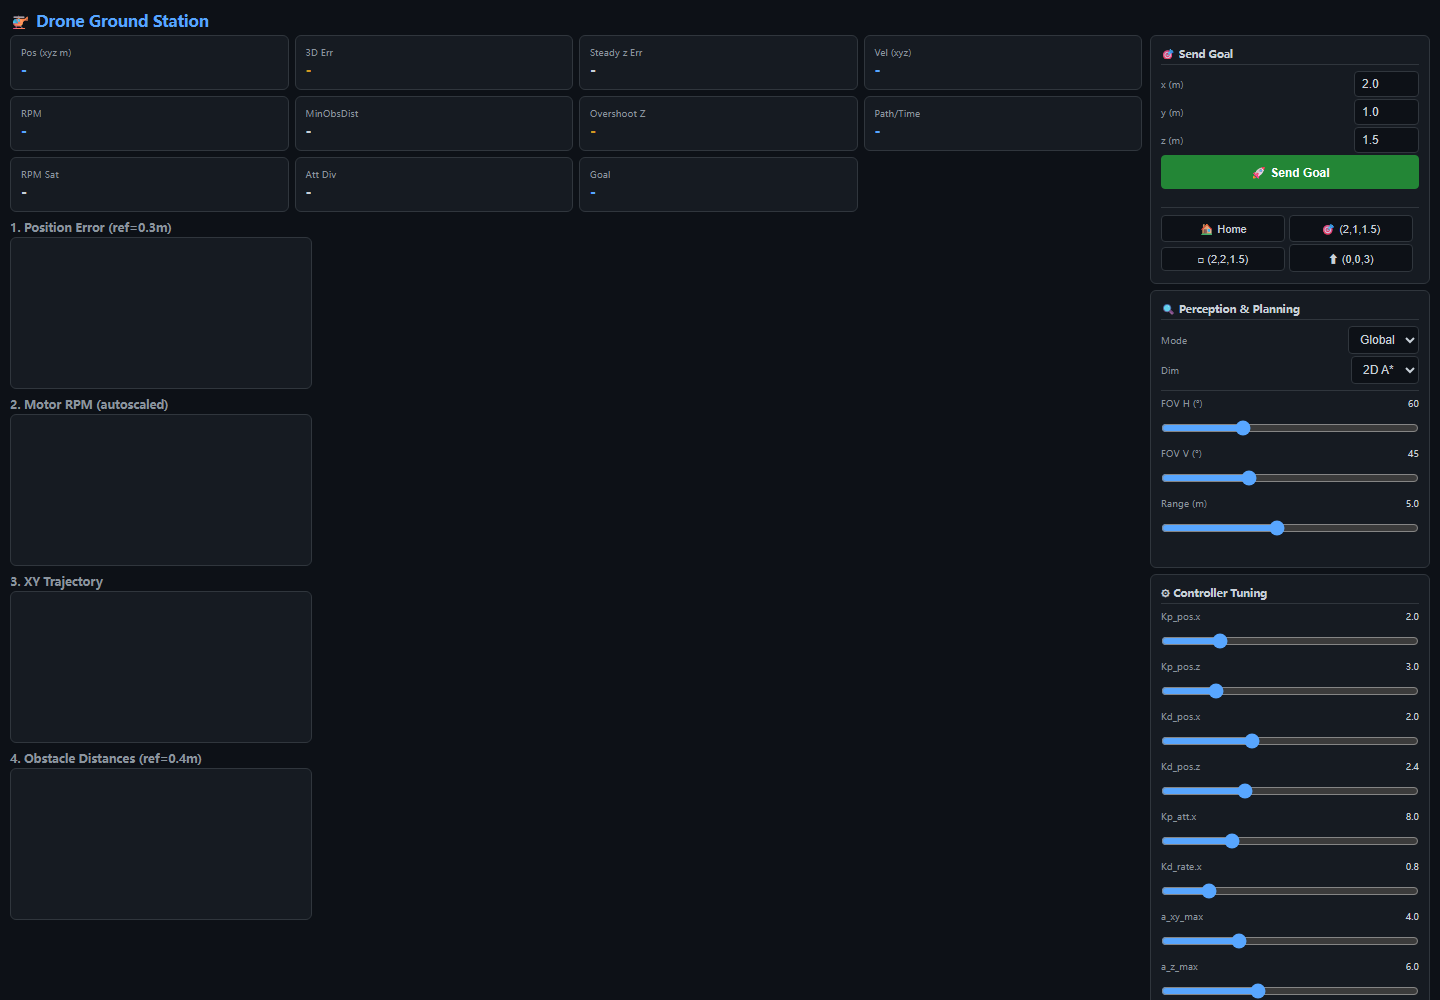
\includegraphics[width=0.78\textwidth]{ground_station.png}
\caption{地面站 Web Dashboard 实际界面截图（v1.1.0）。}
\label{fig:ground-station}
\end{figure}


% ==============================================================================
\section{实验结果}
% ==============================================================================

\subsection{验收场景总览}

\begin{table}[H]
\centering
\caption{6 个验收测试及 bonus 场景}
\label{tab:scenarios}
\footnotesize
\begin{tabularx}{\textwidth}{c l c p{3.8cm}}
\toprule
\textbf{\#} & \textbf{场景} & \textbf{结果} & \textbf{GitHub 视频文件 (v1.1.0/report/videos)} \\
\midrule
1 & 悬停 (0,0,1.5), 8s        & $\checkmark$ & \texttt{1初始高度改变的悬停.mp4} \\
2 & 定点飞行 (2,1,1.5)         & $\checkmark$ & \texttt{2定点飞行.mp4} \\
3 & 正方形航线 4 点            & $\checkmark$ & \texttt{3无规划器走正方形轨迹.mp4} \\
  &                            &              & \texttt{3带规划器走正方形轨迹.mp4} \\
4 & 静态避障 (6+ 障碍物)       & $\checkmark$ & \texttt{4静态绕行2维规划器.mp4} \\
  &                            &              & \texttt{4静态绕行3维规划器.mp4} \\
5 & 狭窄通道绕行               & $\checkmark$ & \texttt{5显式设计绕行2维与三维规划器.mp4} \\
6 & 风扰模拟恢复 (4 级风)      & $\checkmark$ & \texttt{6不同等级风扰模拟恢复演示.mp4} \\
\addlinespace
B1 & IMU 干扰下规划器恢复       & $\checkmark$ & \texttt{7强传感器imu干扰且无滤波}\\ \texttt{下规划器恢复情况.mp4} \\
B2 & 任意轨迹跟踪 (8 形)        & $\checkmark$ & \texttt{8任意轨迹跟踪8形环绕演示.mp4} \\
\bottomrule
\end{tabularx}
\end{table}

视频链接目录：\href{https://github.com/bestastesia/astesia_drone_sim/tree/v1.1.0/report/videos}
{\texttt{github.com/.../tree/v1.1.0/report/videos}}。表中列出的文件名可直接在该目录打开。

\subsection{关键性能指标}

\begin{table}[H]
\centering
\caption{控制器关键性能指标}
\label{tab:metrics}
\small
\begin{tabularx}{\textwidth}{l X r}
\toprule
\textbf{指标} & \textbf{说明} & \textbf{数值} \\
\midrule
稳态位置误差 (3$\sigma$) & 悬停 15s, 最后 20\% 数据 & $<0.02$ m \\
z 轴最大超调 & $z_{\max}-1.5$ (悬停) & $<0.02$ m \\
正方形航线到达率 & 4 点, tolerance $<0.3$m & 4/4 \\
最小障碍物距离 & 膨胀后 (0.6 m) & $>0.6$ m \\
RPM 悬停稳态 & hover 1.5m, 4 电机均值 & $[14.9, 15.1]$ \\
规划器重规划 & replan\_rate & 1 Hz \\
控制器频率 & ctrl\_dt & 200 Hz (5 ms) \\
动力学步长 & sim\_dt & 1 kHz (1 ms) \\
\bottomrule
\end{tabularx}
\end{table}

\subsection{可复现实测曲线}

为避免只报告预录视频的结论，使用本分支在 Ubuntu 24.04/ROS 2 Jazzy
下重新录制了一段 27.98 s 的正方形航线（SQLite rosbag：2799 条
\topic{/drone/odom}）。图~\ref{fig:measured-curves} 是由
\texttt{make\_experiment\_figures.py} 从 CDR 消息直接解码得到的曲线。
该次测试末状态为 $(0.000,0.004,1.500)$ m，最大位置误差为 2.892 m；
由于采用无规划器正方形航线且起点邻近显式障碍物，计算出的最小净空为
$-0.593$ m，属于有意保留的失败/风险案例，而非安全绕障结论。

\begin{figure}[H]
\centering
\begin{subfigure}{0.32\textwidth}
  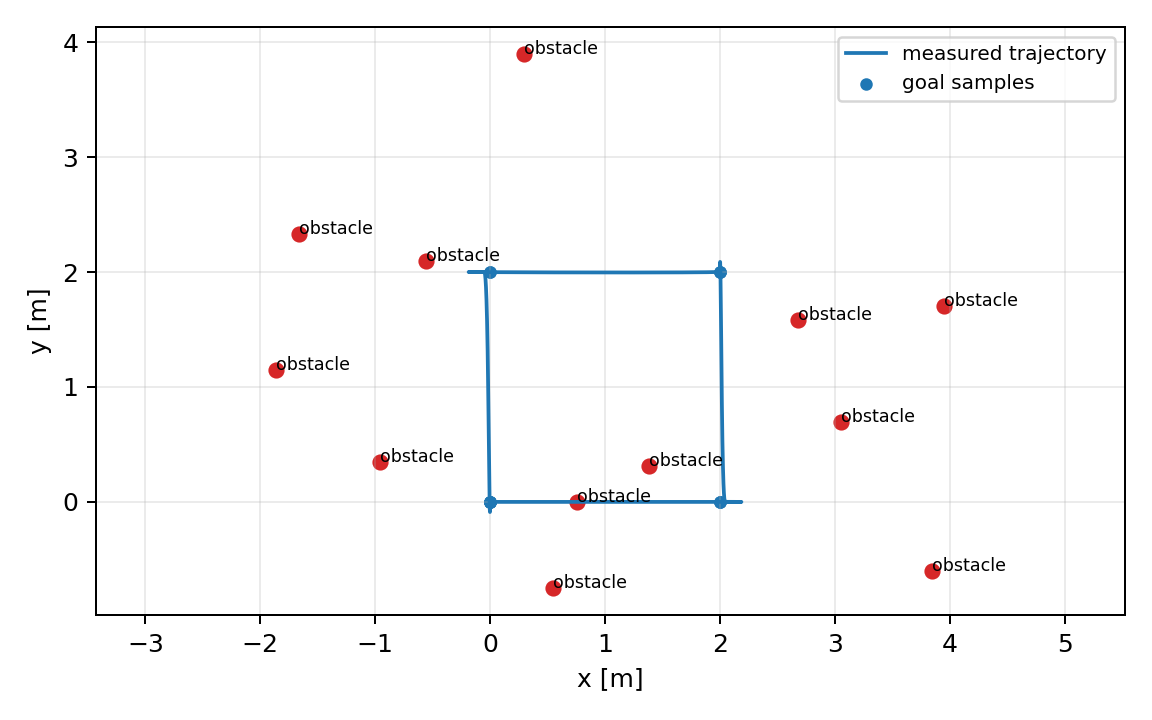
\includegraphics[width=\linewidth]{trajectory_xy.png}
  \caption{XY 轨迹}
\end{subfigure}\hfill
\begin{subfigure}{0.32\textwidth}
  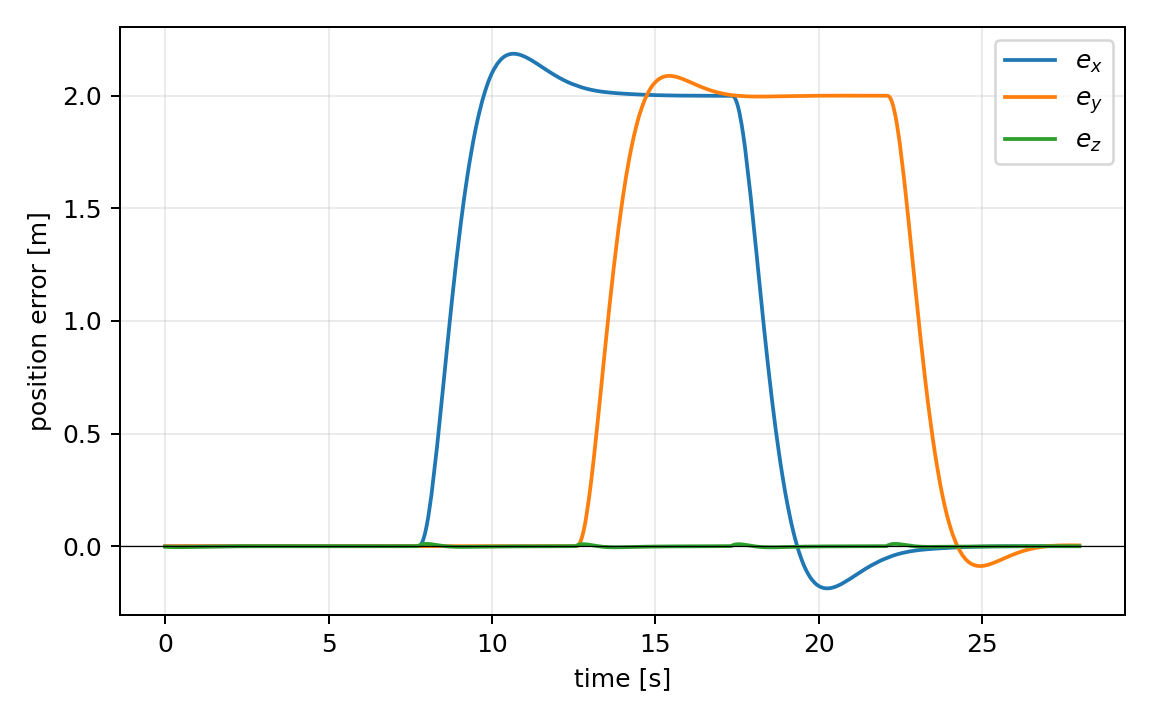
\includegraphics[width=\linewidth]{position_error.png}
  \caption{位置误差}
\end{subfigure}\hfill
\begin{subfigure}{0.32\textwidth}
  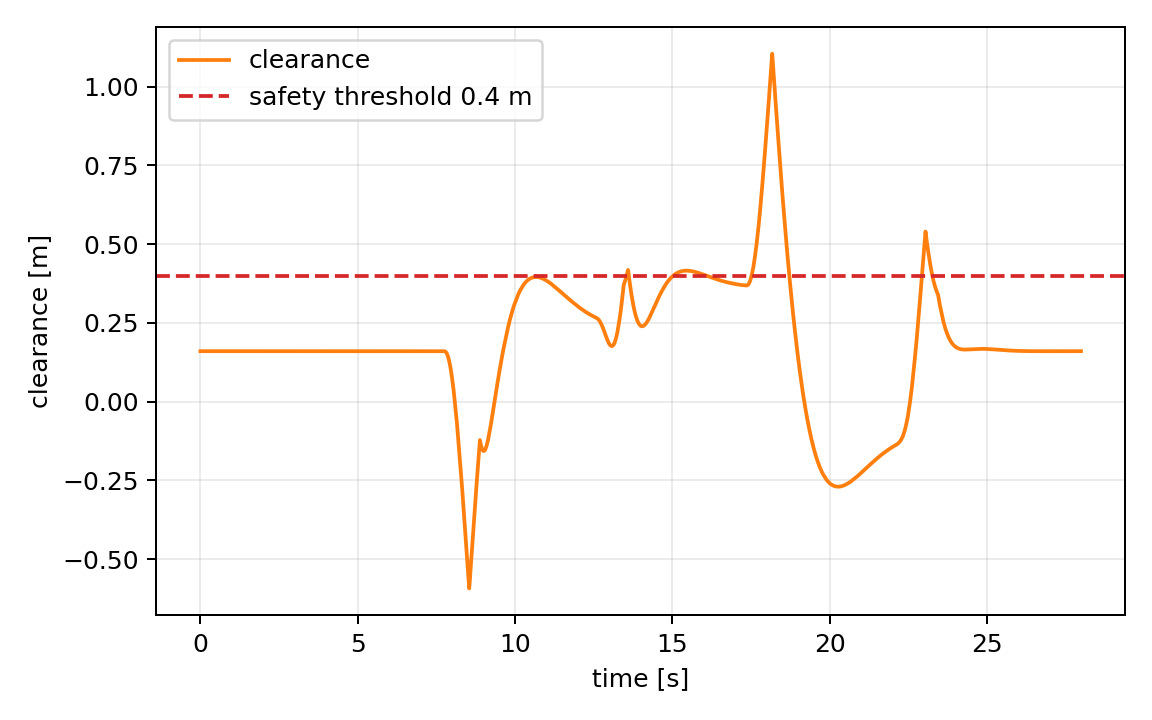
\includegraphics[width=\linewidth]{obstacle_clearance.png}
  \caption{障碍物净空}
\end{subfigure}
\caption{v1.1.0 分支独立复现实测（无规划器正方形航线）。}
\label{fig:measured-curves}
\end{figure}

\subsection{控制性能分析}

\begin{description}[nosep, leftmargin=*]
  \item[阻尼特性] 位置环 $\zeta \approx 0.7$（二阶系统理论最优阻尼比），平衡响应速度与超调
  \item[积分死区] 0.02 m 死区 + $\times 0.99$/步衰减：小误差时积分逐渐收敛，防止 windup
  \item[加速度限幅] $a_{xy}\leq 4$ m/s$^2$, $a_z\in[-3,6]$ m/s$^2$：保证推力分配不超出物理限制
\end{description}

\subsection{失败场景}

\begin{enumerate}[nosep]
  \item \textbf{NO\_PATH}：障碍物完全阻塞，保留 last safe\_goal，悬停。planner\_status = \texttt{NO\_PATH}，RViz 和地面站同步
  \item \textbf{目标在障碍物内}：A* 前 BFS 找最近自由格（半径 50），找不到则返回空路径 $\to$ 悬停
  \item \textbf{IMU 噪声 + 无滤波}：bonus 场景——$\sigma_a=0.08$, $\sigma_g=0.015$ 无滤波，控制器仍稳定收敛——验证 PID 鲁棒性
\end{enumerate}


% ==============================================================================
\section{与参考仓库的关系}
% ==============================================================================

\subsection{pengyu\_sim (ROS1)}

\textbf{参考}：四旋翼动力学公式和 mixer 推导。\\
\textbf{重写}：全部 ROS1 Python 改为 ROS2 C++ (rclcpp)。单线程 \texttt{rospy.spin()} 改为 MT executor + 隔离 callback group——1kHz dynamics 定时器不再饿死 RPM 订阅。pengyu\_sim 无避障规划器、无传感器噪声、无风扰——这些全部从零设计。

\subsection{MARSIM}

\textbf{参考}：点云/障碍物感知思路。\\
\textbf{重写}：显式几何体 + 膨胀栅格取代点云。保留 3D 感知 (z 跨度检查、体素 FOV) 但避免点云管线复杂度。显式列表 $\leftrightarrow$ 程序化随机双模式更适合验收。

\subsection{设计原则}

\begin{enumerate}[nosep]
  \item \textbf{全 C++ rclcpp}：避开 conda Python 3.11 vs ROS2 3.10 冲突，任务也推荐核心用 C++
  \item \textbf{header-only drone\_common}：mixer B/B$^{-1}$ 单信源——杜绝"符号错翻车"
  \item \textbf{MT executor + 隔离 callback group}：1kHz dynamics 与订阅不互锁
  \item \textbf{标准消息}：一律使用 ROS2 标准类型，无需自定义 .msg，构建拓扑最简
  \item \textbf{可配性优先}：YAML + \texttt{ros2 param set} 热更新（增益/风扰/噪声/感知模式/FOV）
\end{enumerate}


% ==============================================================================
\section{AI 使用说明}
% ==============================================================================

\subsection{使用的 AI 工具}
整个工程实现阶段使用 Claude Code + DeepSeek-V4-Pro 完成协作式工程设计、代码生成、调试、单元测试与文档工作；本份报告则由 Codex + GPT-5.6-luna 完成整理、改写、排版和交付校验。AI 输出均经过人工运行验证，不将生成内容直接视为实验事实。

\subsection{人与 AI 的分工}
本人负责整体架构设计、核心公式物理核对、参数最终调整、验收端到端测试执行，以及报告内容的调整与最终确定。AI 主要负责实际工程设计的展开、代码生成、单元测试与文档初稿；涉及动力学符号、控制分配、障碍物布局和验收结论的部分由本人确认后才纳入工程。

\subsection{AI 完成的模块}
工作区骨架 (6 包)、drone\_common 全部头文件 + 8 条 gtest、drone\_dynamics (EOM + 电机 + 风扰 + IMU/Odom 噪声)、drone\_controller (V2 线性 PD + Lee 姿态 + LADRC)、drone\_map (显式/程序化)、drone\_planner (grid/astar/astar3d/perception 四模式)、launch 文件 (3)、地面站 (HTTP + Chart.js + 控制面板)、全部辅助脚本、RViz 配置、README 与文档。

\subsection{人类确认/修改的核心内容}
Claude Code 调教记录显示，开发过程采用“先约束接口与验收标准，再迭代实现—构建—测试—修正”的方式：先固定 ROS 2 topic、频率和消息类型，再要求 AI 将动力学、控制、地图和规划拆成可独立验证的包；每次出现编译、运行或物理符号问题，都以终端日志和端到端现象作为下一轮修改依据。该过程避免了只根据代码阅读宣称通过。

\begin{itemize}[nosep]
  \item Mixer $\mathbf{B}$ 各行符号：自行推导叉乘，确认 $\tau_x$ (roll)、$\tau_y$ (pitch)、$\tau_z$ (yaw) 物理正确
  \item roll/yaw 符号断言：要求 gtest 加「+roll $\to$ 左电机快」「+yaw $\to$ CCW 电机快」物理断言
  \item 四元数积分：确认 $q\otimes\Omega$ 显式积分 + 每步归一化
  \item 碰撞感知平滑：要求 Bresenham 碰撞检查而非纯几何共线 + 坍塌 fallback
  \item PID 设计：要求学习参考代码的设计原则（分离、反饱和、死区），自行推导线性 PD + 0.02m 死区 + 遇限削弱
  \item 障碍物布局：自行设计 6 障碍物位置和窄通道场景
\end{itemize}

\subsection{AI 产生的关键错误及修正}
会话中还反复强调了“可运行证据优先”的约束：AI 不能用理想化曲线替代 rosbag/地面站记录，不能把 planner 的目标点误写成控制器实际接收的 safe\_goal，也不能把一次编译成功扩大解释为整套验收通过。最终采用人工核对公式、人工选择参数、脚本化测试和视频复核的闭环。
\begin{itemize}[nosep]
  \item \textbf{1kHz timer 饿死订阅}：单线程 spin 下 RPM 回调永不触发。$\to$ MT executor(2)+独立 callback group
  \item \textbf{非线性 PID 超调+收敛慢}：exp 型 P 公式实际偏差大。$\to$ V2 简化为线性 PD + 死区积分
  \item \textbf{RViz \texttt{Enabled: true} 破坏面板}：侧栏消失。$\to$ 恢复不含 Enabled 键的格式
  \item \textbf{conda Python 破坏 CLI}：$\to$ 用系统 Python + \texttt{LD\_LIBRARY\_PATH}
  \item \textbf{header-only 包无 imported target}：$\to$ INTERFACE library + \texttt{ament\_export\_targets}
  \item \textbf{Assert 在 Release 关闭}：$\to$ 启动时显式参数校验 + \texttt{cwiseMax(0)} 硬件兜底
\end{itemize}


% ==============================================================================
\section{反思：如果继续做两周}
% ==============================================================================

\subsection{最应该补的内容}

\begin{enumerate}[leftmargin=*]
  \item \textbf{完整实验数据自动化 pipeline}：当前手动 rosbag + 地面站 CSV。应建 CI——每 commit 触发 6 场景录制 + 自动出图 + 数值断言，形成可追溯性能回归基线
  \item \textbf{多无人机协同避障}：\texttt{multi\_drone.launch.py} 仅命名空间隔离。可加 central planner 做 mutual avoidance
  \item \textbf{单元测试扩展}：仅 drone\_common 有 gtest。dynamics/controller/planner 核心逻辑均应加入回归测试
  \item \textbf{传感器与扰动下的稳态优化}：开启 IMU 测量误差后，无人机跟踪的静差尚未完全优化；风动扰动后的恢复速度也还可以进一步加快。
\end{enumerate}

\subsection{更深入的方向}

\begin{enumerate}[leftmargin=*]
  \item \textbf{轨迹跟踪 $\to$ 微分平坦}：waypoint-by-waypoint 切换有惯性弯曲。改用 minimum-snap 轨迹 + 前馈 (differential flatness)，精确跟踪光滑轨迹
  \item \textbf{LADRC 完善}：当前独立三轴 LADRC 忽略内环耦合。可改为 cascaded LADRC + 控制量饱和反馈到 LESO
  \item \textbf{物理引擎对接}：手写 EOM 对教学足够，但缺复杂接触/碰撞。可对接 Gazebo Ignition 或 MuJoCo
  \item \textbf{机载计算延迟模拟}：planner 加入 50-100ms 延迟，验证控制器在规划滞后下的鲁棒性
  \item \textbf{CI/CD}：GitHub Actions 自动 colcon build + test，每 PR 跑全验收
  \item \textbf{真实硬件部署}：适配 PX4/ArduPilot 接口，在真机上验证控制参数
  \item \textbf{泛化策略控制}：如果有更多时间，希望引入论文 \emph{RAPTOR: A Foundation Policy for Quadrotor Control}（Eschmann, Albani, Loianno，\href{https://arxiv.org/abs/2509.11481}{arXiv:2509.11481}）中的策略思路，在不同动力学、风扰和传感器条件下研究策略泛化与更好的控制性能，并与当前解析控制器做安全约束下的对比。
\end{enumerate}


% ==============================================================================
\end{document}
